\documentclass[10pt, onecolumn, draftclsnofoot, letterpaper, compsoc]{IEEEtran}

\usepackage{graphicx}
\usepackage{amssymb}
\usepackage{amsmath}
\usepackage{amsthm}
\usepackage{alltt}
\usepackage{color}
\usepackage{url}
\usepackage{minted}
\usepackage{hyperref}
\usepackage{geometry}

\graphicspath{ {images/} }
\geometry{textheight=8.5in, textwidth=7in}

\renewcommand*\contentsname{Table of Contents} % Rename ToC

% Temp title and author
\title{Midterm Progress Report}
\author{Totality AweSun \\
		Bret~Lorimore, Jacob~Fenger, George~Harder \\
		\textit{May 15, 2017 \\
		CS 463 - Spring 2017}}

\begin{document}

\maketitle

\begin{abstract}
This document describes the current state of the \textit{North American Solar Eclipse 2017}
senior capstone project. The document gives a brief overview of the project and its components,
describes the current state of the project, describes problems that have been
encountered throughout the term, shows some of the code that has been produced thus far, gives
a week-by-week outline of progress throughout the term, and reflects over the term in the
retrospectives section at the end.
\end{abstract}

\newpage

\tableofcontents

\newpage

%%%%%%%%%%%%%%%%%%%%%%%%
%   Project Overview   %
%%%%%%%%%%%%%%%%%%%%%%%%
\section{Project Overview}

The North American Solar Eclipse 2017 Senior Capstone project is partnered
with Google to build a set of applications that will assist the development of
the Eclipse Megamovie Project. The overall project has been broken down into
three components: the eclipse image processor, the image processor manager, and
the solar eclipse simulator. Each will be individually outlined in the sections
below. \\

\subsection{Image Processor}

The image processor’s primary activity is to quickly and consistently identify
images of an eclipse at totality. The Eclipse Megamovie project will be
collecting thousands of images from photographers around the country, and the
image processor needs to identify the images of the eclipse at totality so that
these can then be stitched into a timelapse movie. In order to make the
stitching as easy as possible for the Eclipse Megamovie team, the image
processor will add metadata to each processed image that includes spatial
information about where the image was taken along the path of totality and
temporal information about how far into totality the eclipse is.


The purpose of the Image Processor is not to process many images as quickly as
possible. Instead, our goal is to be able to consistently and accurately process
a single image at a time. As such, the image processor will fit into the larger
project as an executable file that is called by the Image Processor Manager.
This allows us to focus the image processor solely on a single goal, and leave
parallelization and deployment to a different piece of the project. \\

\subsection{Image Processor Developer Pipeline}

The image processor developmer pipeline is a tool that will assist any future
development of the image processor. It consists of a script that operates
several primary stages that provides developers with an easily manipulatable
interface to the image processor. The script first downloads images from a
Google Cloud Storage (GCS) bucket. Then it runs the images through the image
processor in one of two modes: "batch" or "window." The first mode runs through
all of the images at once and the second lets the user see the results of a run
one image at a time. After the image processor finishes running and writing its
output, the script then uploads all of the processed images and the output into
a GCS bucket so the information can be easily found and reviewed. Lastly, the
pipeline calls a python script that formats the output of the image processor
into an HTML document. The HTML document contains metadata about the run of the
image processor so that runs can be recreated and easily compared. In addition,
it has a table with information about each individual image processed in the run.

The image processor developer pipeline is a valuable tool because it gives
developers very fine control over runs of the image processor. The script that
runs the pipeline takes arguments that control the mode, where to download
images from, where to upload the to, and what paramters to pass to the image
processor. This allows developers to easily experiment with small and large
changes to the image processor and examine results. \\

\subsection{Eclipse Simulator}

The eclipse simulator is an independent JavaScript module that has been
added to the existing Eclipse Megamovie webpage. This simulator will allow
users to "preview" a 2D stylized depiction of the eclipse from a given location
in the United States. Users interact with the simulator using a time slider
that ranges from 1.5 hours before to 1.5 hours after the eclipse, a "play" button,
location selection via a map or search bar, and a zoom mode.

To help with the eclipse ephemeris computations, we used an external
JavaScript library called MeeusJs. For the front end view for the simulator,
we utilized HTML5 SVG. Our eclipse simulator uses a model-view-controller 
architecture for controlling the states of each component as well as handling
the interactions. This architecture was chosen due to the ability to easily
exchange a component without altering the whole design of the system. For
example, if one wanted to create a whole new front end for the simulator,
they would not need to rewrite the model or controller component of the system.
They would simply need to ensure that the new view component can handle the
interactions with the controller module. \\

\subsection{[SUPPLEMENTAL] Eclipse Image Classifier}

We have agreed to continue working with our client beyond expo, until graduation.
After completing work on the Image Processor and Developer Pipeline, he
requested that we begin working on an image classifier to classify images as being of
total solar eclipses or not. This work is entirely supplemental to our project, as
our client did not even request that we work on it until after the May 1st code freeze.
As such, it is not described in our requirements or design document. We do however, in this
document, give a brief summary of work on this project component.

This classifier will be used to weed out non-totality images before they are fed into the
Image Processor. This allows the Image Processor to be specifically tailored to images
of totality -- simlifying its implementation and improving its accuracy. \\

%%%%%%%%%%%%%%%%%%%%%%%%
%   Current Status     %
%%%%%%%%%%%%%%%%%%%%%%%%
\section{Current Status of the Project}

Based on the requirments we set for ourselves and agreed upon with our sponsor
our project is effectively complete. We have delivered a solar eclipse simulator
that meets the specifications our sponsor requested. In addition, we have
produced an image processing development pipline that will assist in future
development of our image processor. \\

\subsection{Image Processor}

As of the code freeze on May 1, we had a working image processor that identified
circles in images of eclipses and drew the two most prominent circles
(ostensibly the sun and moon) over the image. This tool meets ours and our
sponsor's specifications for the image processor. In addition, during meetings
with our sponsor he has expressed the fact that he is happy with our work and
appreciates what we have done. \\

\subsection{Image Processor Developer Pipeline}

The image processor developer pipeline meets the specifications our client
requested for a platform that will aid in future development of the image
processor. The developer pipeline is a tool that allows developers to quickly
and easily run and experiment with different paramaters or tweaks to code. This
tool gives our sponsor, who plans to continue development on the image processor,
an effective way to validate his development is improving the image processor. \\

\subsection{Eclipse Simulator}

The eclipse simulator we delivered to our sponsor and his team has met the
requirements we set forth and is now live on the eclipsemega.movie website. The
eclipse simulator has exceeded our expectations for quality and our sponsor has
expressed his pleasure with our finished product. \\

\subsection{[SUPPLEMENTAL] Eclipse Image Classifier}

The eclipse image classifier is a supplemental piece of the project that our
sponsor asked us to investigate with the remaining time we had on the project.
Currently, we are looking into using Google Cloud Vision (GCV) to classify images
as either partial or total eclipse. This is because we and our sponsor have
decided to add a precondition of the image processor that the images it works
on are of a total eclipse. By using GCV to classify images, we can meet this
precondition. \\

%%%%%%%%%%%%%%%%%%%%%%%%
%   Problems           %
%%%%%%%%%%%%%%%%%%%%%%%%
\section{Problems and Possible Solutions}


%%%%%%%%%%%%%%%%%%%%%%%%
%   Things Left to Do  %
%%%%%%%%%%%%%%%%%%%%%%%%
\section{Things Left to Do}

\subsection{Image Processor}

Lorem \\

\subsection{Image Processor Developer Pipeline}

Lorem \\

\subsection{Eclipse Simulator}

None! \\


%%%%%%%%%%%%%%%%%%%%%%%%
%   Code               %
%%%%%%%%%%%%%%%%%%%%%%%%
\newpage
\section{Interesting Code}

This is a derived image processor pipeline that overrides the image preprocessing
to make it use erosion/dilation. This improves image processor performance by approx. 4-20\%
on various datasets. \\

\begin{minted}{cpp}
class DilationPipeline : public ImgProcPipelineBase {

public:
    DilationPipeline(int argc, char **argv) : ImgProcPipelineBase(argc, argv) {};

    virtual void preprocess(const cv::Mat &image, cv::Mat &processed)
    {
        Mat blurred;
        std::pair<int, int> dimensions;

        // Record the time it takes to preprocess an image
        time_t t = std::clock();

        // Convert image to black and white if it is not already
        if (image.channels() != 1)
        {
            cvtColor(image, processed, CV_BGR2GRAY);
        }
        else
        {
            processed = image.clone();
        }
        // Resize image to normalized size
        dimensions = getRescaledDimensions(processed, HD_MAX_W, HD_MAX_H);
        resize(processed, processed, Size(dimensions.first, dimensions.second));

        this->current_image.add_intermediate_image("gray", processed);

        // Erosion/dilation kernel
        Mat kernel = getStructuringElement(MORPH_RECT, Size(5, 1));

        // Erosion
        erode(processed, processed, kernel);
        this->current_image.add_intermediate_image("erode", processed);

        // Dilation
        dilate(processed, processed, kernel);
        this->current_image.add_intermediate_image("dilate", processed);

        GaussianBlur(processed, processed, Size(9, 9), 30, 30);
        this->current_image.add_intermediate_image("blur", processed);

        t = std::clock() - t;

        // add execution time
        this->current_image.add_execution_time(
		    "preprocess", (double) t / (double) CLOCKS_PER_SEC
        );
    }
};
\end{minted}

\newpage
\section{Screenshots}

\begin{figure}[!h]
	\begin{center}
  		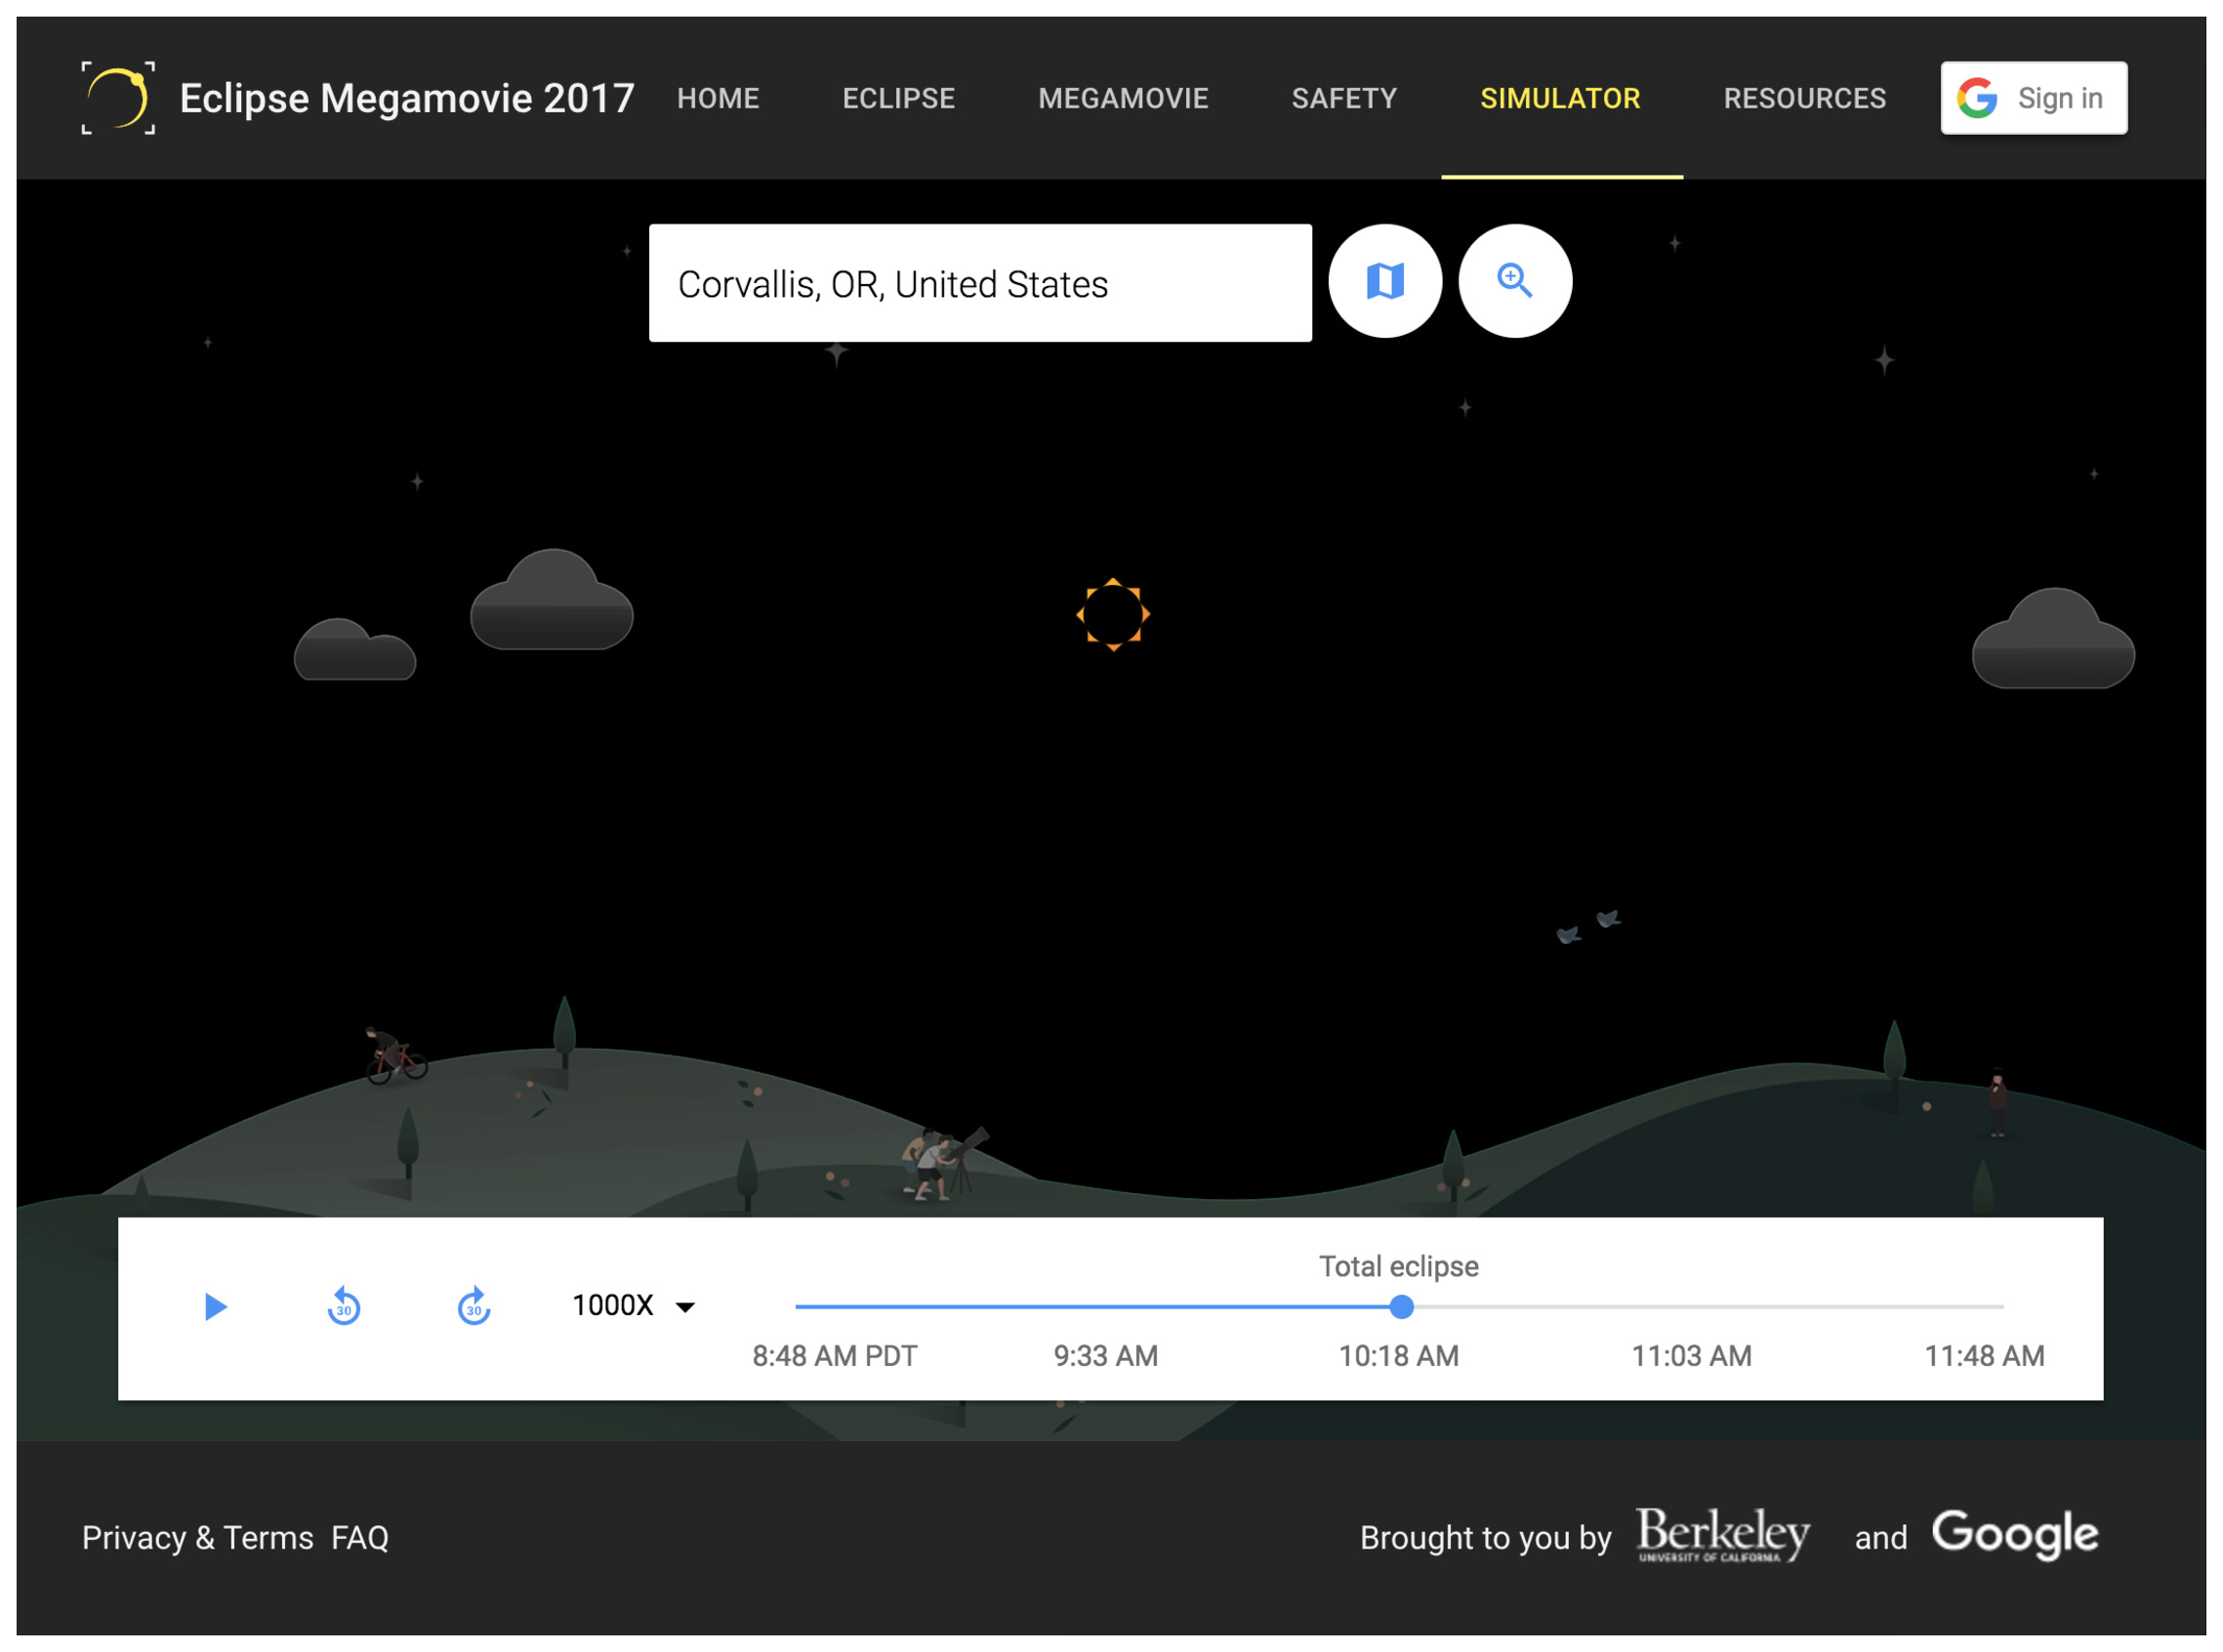
\includegraphics[width=\textwidth]{sim_total.eps}
		\caption{Simulator in wide mode showing a total solar eclipse}
	\end{center}
\end{figure}
\newpage

\begin{figure}[!h]
	\begin{center}
			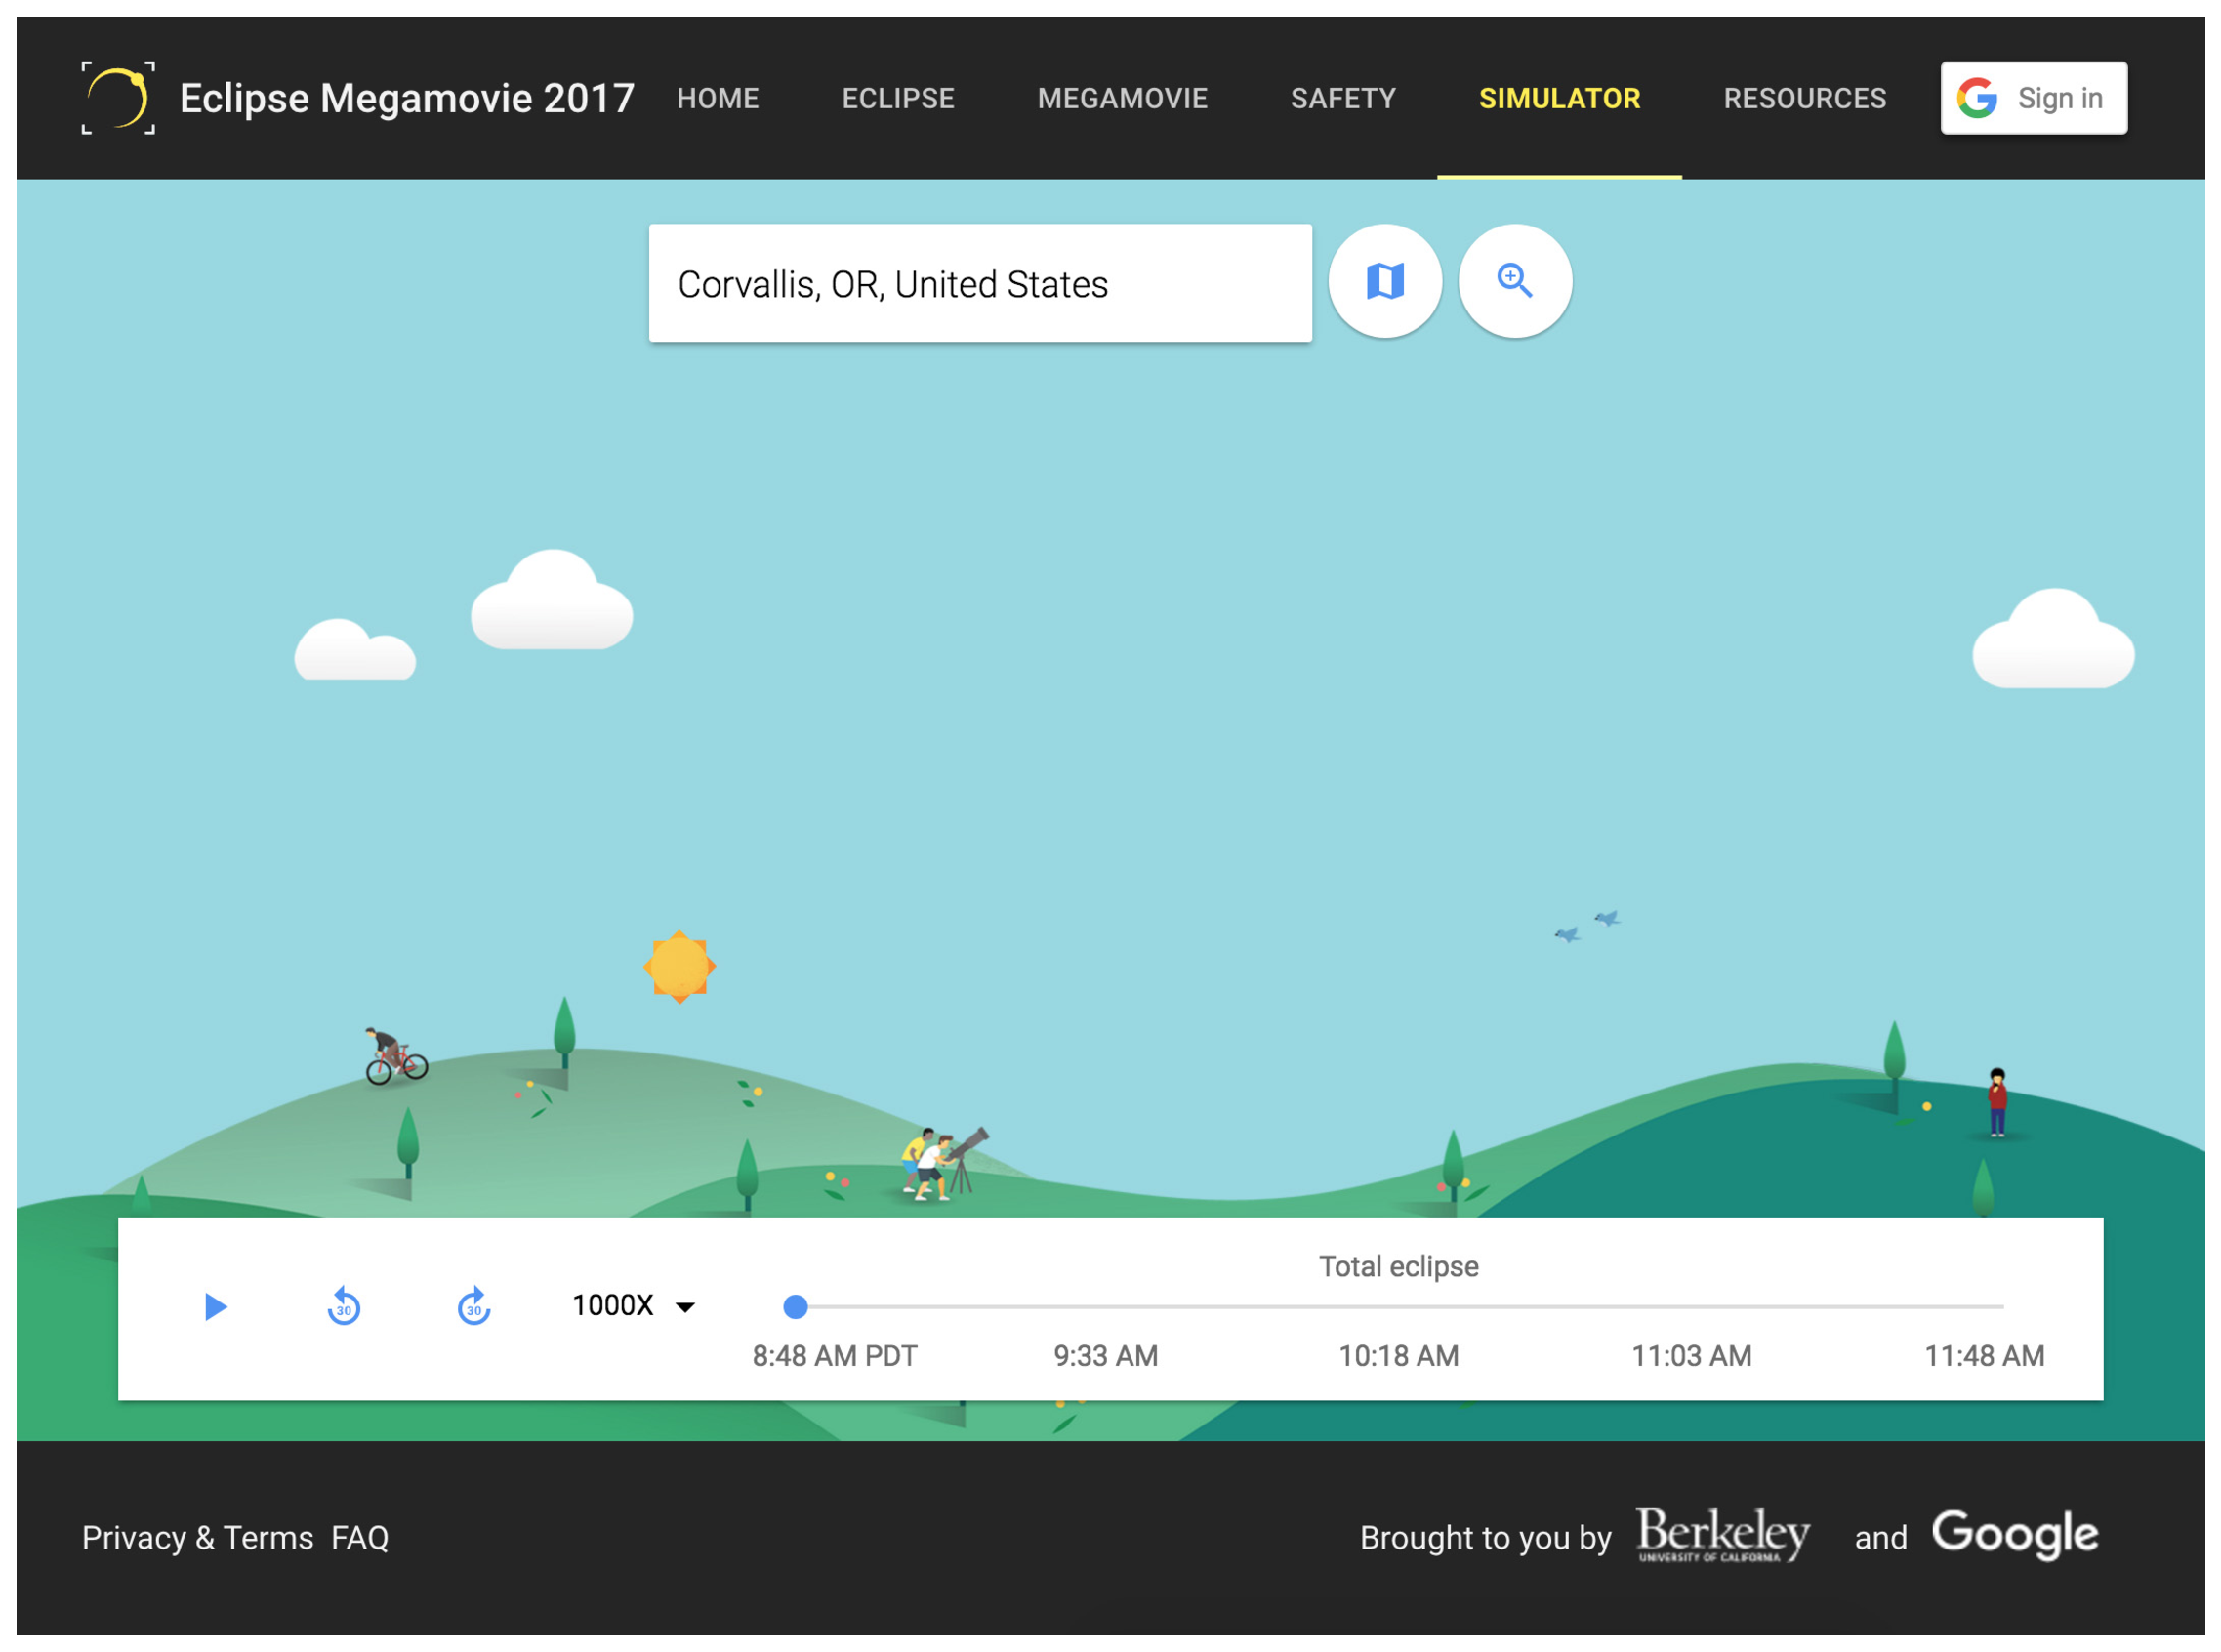
\includegraphics[width=\textwidth]{sim.eps}
		\caption{Simulator in wide mode showing no eclipse}
	\end{center}
\end{figure}
\newpage

\begin{figure}[!h]
	\begin{center}
			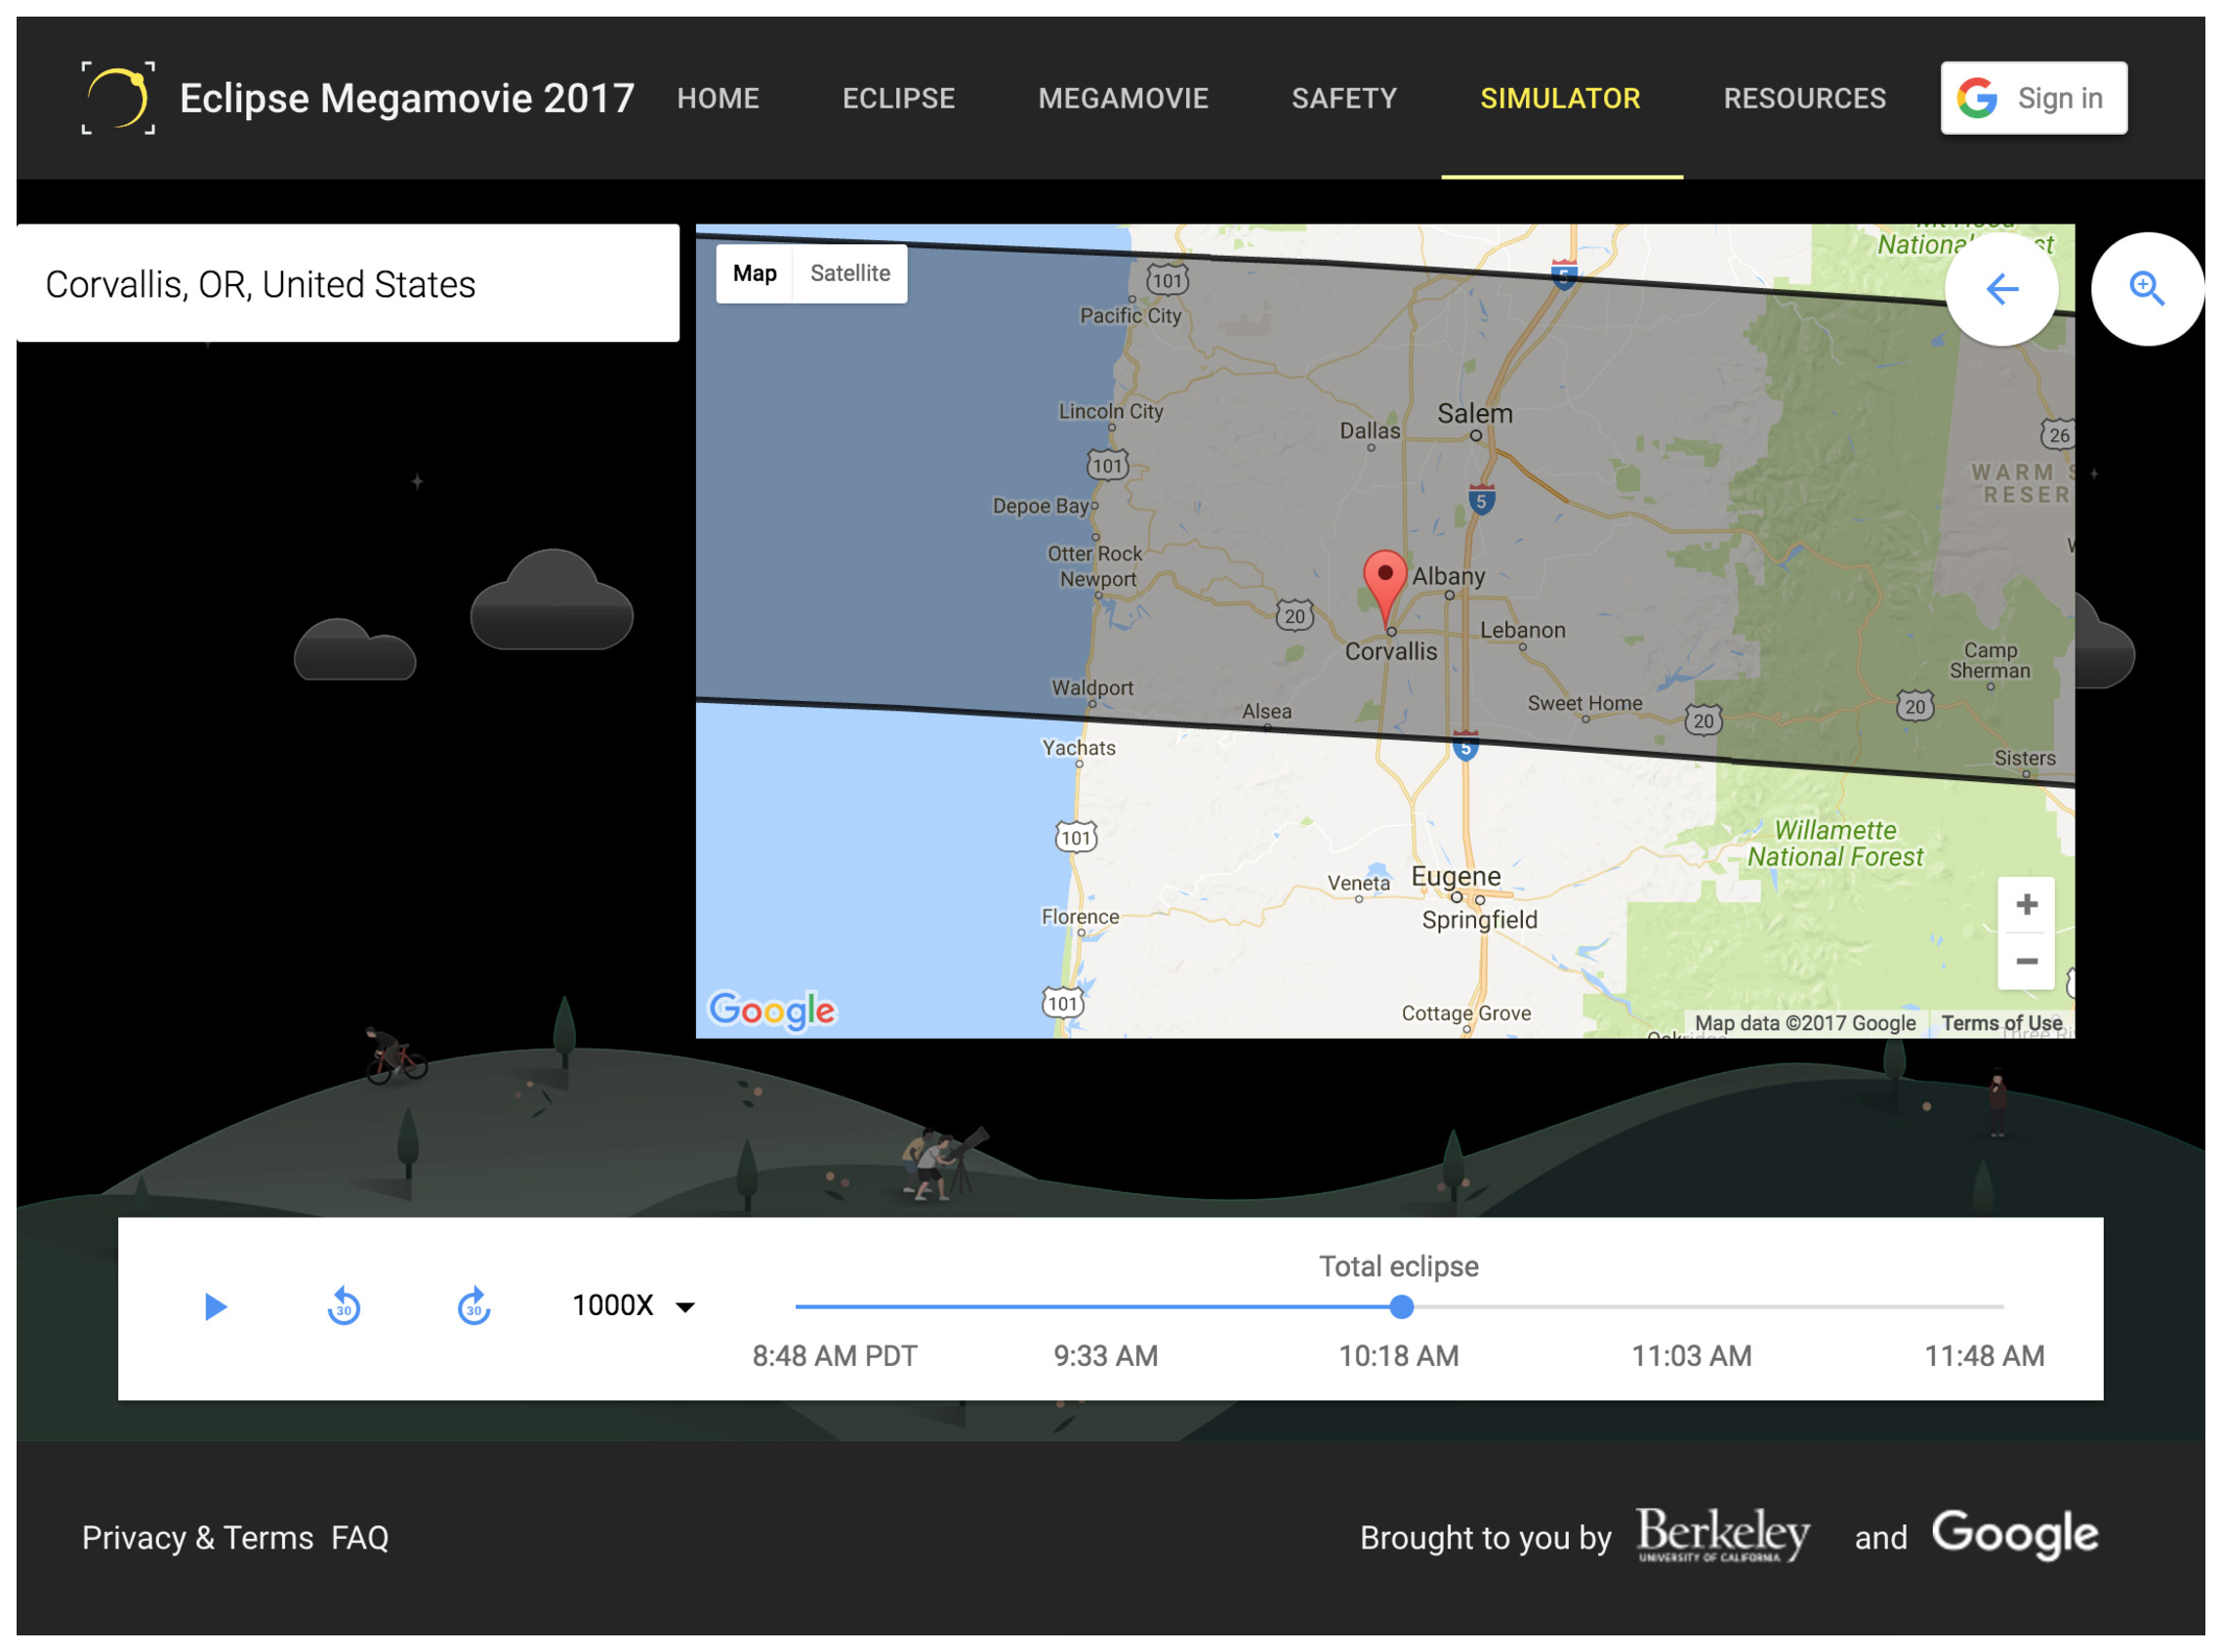
\includegraphics[width=\textwidth]{sim_map.eps}
		\caption{Simulator with map expanded}
	\end{center}
\end{figure}
\newpage

\begin{figure}[!h]
    \begin{center}
            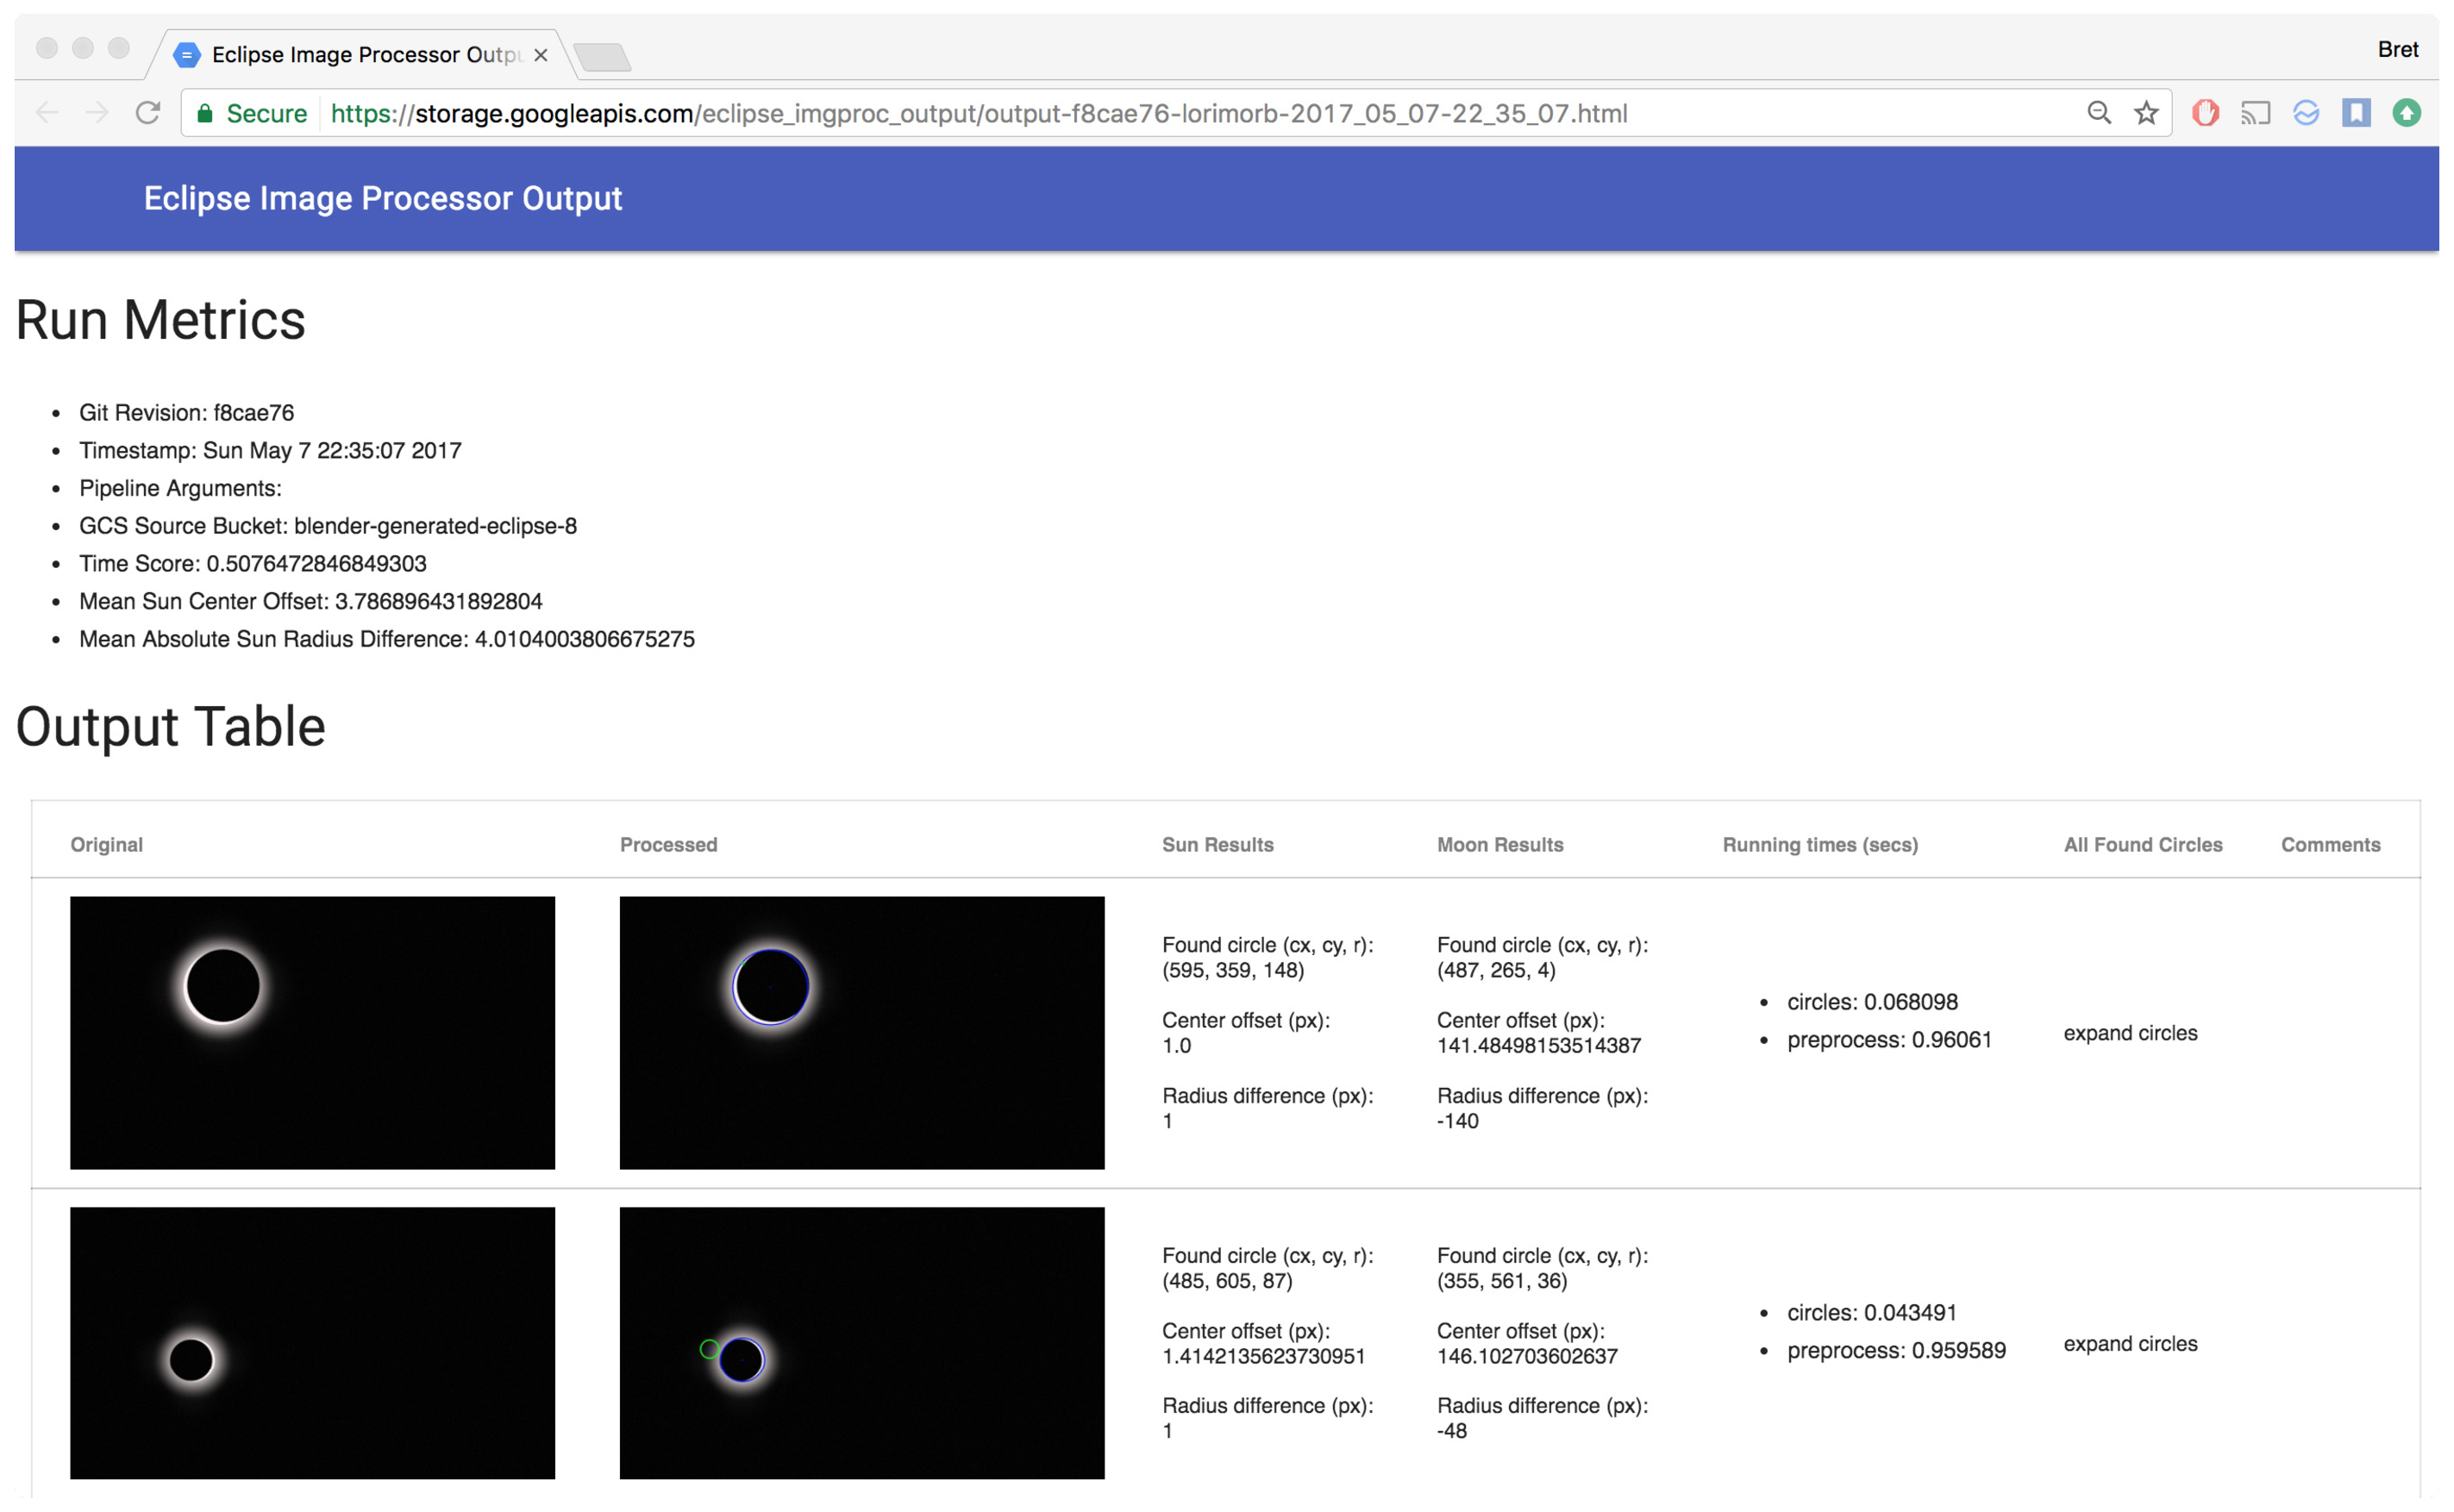
\includegraphics[width=\textwidth]{imgproc.eps}
        \caption{Image Processor Developer Pipeline Results File}
    \end{center}
\end{figure}
\newpage


%%%%%%%%%%%%%%%%%%%%%%%%
%   Weekly Summary     %
%%%%%%%%%%%%%%%%%%%%%%%%
\newpage
\section{Week by Week Summary of Group Activities}

\subsection{Week 1}

    \begin{itemize}

	\item Simulator launched!!@\&\% See it at \href{https://eclipsemega.movie/simulator}{https://eclipsemega.movie/simulator}.

	\item Began refactor of image processor pipeline to be a class that can easily be inherited from to build different image processor implementations.

	\item Started refactoring the image processing code that Bret wrote during his internship.

	\item Added ability for \texttt{output.html} table to be sorted by column on a click.
		\begin{itemize}
			\item User can sort in ascending or descending order on four different columns.
			\item Sorting algorithm is currently very naive because it made DOM manipulations easy, going to improve this.
		\end{itemize}

    \end{itemize}

\subsection{Week 2}

    \begin{itemize}

	\item Completed image processor refactor.

	\item Revised 1st poster draft.

	\item Submitted expo model release.

	\item Updated \texttt{run\_imgproc\_test} tool to upload processed images and html output file to Google Cloud Storage.

	\item Improved \texttt{output.html} sorting algorithm.

		\begin{itemize}
			\item Reworked sorting to use JavaScript Array.sort instead of DOM manipulation.
			\item Wrote a comparator for each column that parses each cell's content and performs a comparison.
			\item The rows are converted from an HTML collection to a JavaScript array before sorting, are sorted, then are attached back to the DOM.
		\end{itemize}

		\item Altered output.html generation script to handle new input file format.

		\begin{itemize}
			\item Changed some columns in the data table to work with new data.
		\end{itemize}

    \end{itemize}

\subsection{Week 3}

    \begin{itemize}

	\item Updated image processor to use GFlags for command line arg parsing.

	\item Added command line arguments for several Hough transform parameters following request from client.

	\item Updated test bash script in \texttt{run\_imgproc\_test} to accept flags to be passed to the image
	processing pipeline. Additionally, these are added to the output HTML file so that it is easy to exactly
	reproduce a run of the tool.

	\item Ran image processor on all images that our client has uploaded to Google Cloud Storage, forwarded results
	to him.

	\item Brainstormed "jitter" method for small adjustments to circles found by \texttt{cv::HoughCircles}.

	\item Requested eclipse glasses from Google Making \& Science Team team to hand out at expo.

	\item Reviewed/merged pull request \#16 from Justin.

	\item Fixed several issues and added features to the output generation script.

	\begin{itemize}
		\item Made the script tolerant to not having a hand labeled ground truth file.
		\item Made the script handle cases where no circles are found.
		\item Added a column so that all circles found in an image can be displayed if a user clicks on that cell.
		\item Added scores for both timing an accuracy that can be used as single metric to compare runs.
	\end{itemize}

    \end{itemize}

\subsection{Week 4}

    \begin{itemize}

	\item Experimented with erosion/dilation for image processor preprocessing.

	\item Ran image processor on large set of automatically generated (using blender) images ground truth.

	\item Fixed a couple bugs in the image processor.

	\begin{itemize}
		\item Circles were not scaled up when saved to metadata.txt if the working image was smaller than the original.
		\item Circles rendered on PNGs with an alpha channel appeared transparent. Changed image processor to open images in "color" mode, discarding PNG alpha channels.
	\end{itemize}

	\item Worked with Google/Berkeley team on minor set of simulator improvements.

	\item Met with another group to finalize our poster and to do a peer review. In addition, we received usage statistic regarding the simulator for our poster.

	\item Took team photo for poster, made final changes to poster, got it approved by client!

	\item Updated requirements to more closely match what we ended up doing, specifically with regard to the image processor, got them approved by client!

	\begin{itemize}
		\item Our client treated us similar to an internal software dev team and told us what he'd like done in a bit of an ad-hoc fashion. This worked really well, it just resulted in or requirements having to evolve.
	\end{itemize}

	\item Refined the output generation script based on client feedback.

    \end{itemize}

\subsection{Week 5}

    \begin{itemize}

	\item Incorporated erosion/dilation into image processing pipeline.

	\begin{itemize}
		\item Ran comparison of image processor performance using \texttt{ImgProcPipelineBase} and
		\texttt{DilationPipeline}. \texttt{DilationPipeline} performed well, exceeding \texttt{ImgProcPipelineBase}
		overall, with one outlier.
	\end{itemize}

	\item Finalized simulator tweaks.

	\item Fixed a sorting error in the sun diff comparator.

	\begin{itemize}
		\item The comparator was not accounting for cases where there was no ground truth, now fixed.
	\end{itemize}

	\item Submitted the final draft of our poster for printing.

	\item Completed the WIRED review assignments.

    \end{itemize}

\subsection{Week 6}

    \begin{itemize}

	\item Lorem

    \end{itemize}

\newpage
\section{Retrospectives}

\begin{table}[!h]
    \centering
    \begin{tabular}{|p{.3\linewidth}|p{.3\linewidth}|p{.3\linewidth}|}

    \cline{3-3}

    \hline \textbf{Positives} & \textbf{Deltas} & \textbf{Actions} \\ \hline

    Simulator completed and launched & & \\ \hline

	Completed Image Processor & & \\ \hline

	Completed Image Processor Developer Pipeline & & \\ \hline

	 & Supplemental Image Classifier has poor performance (approx. 70\% test accuracy) & Collect/label more data, update model as necessary \\ \hline

    \end{tabular}
\end{table}

\end{document}
